\chapter{Systems of ODEs}
\label{systems}

In the previous chapter we used Euler's method and {\tt ode45} to solve a single first-order differential equation.  In this chapter we'll move on to systems of ODEs and implement a model of a predator-prey system.  But first, we have to learn more about matrices.


\section{Matrices}

A \emph{matrix} is a two-dimensional version of a vector.  Like a vector,
it contains elements that are identified by indices.  The difference
is that the elements are arranged in rows and columns, so it takes
{\em two} indices to identify an element.

\subsection{Creating a Matrix}

\index{matrix}
\index{index}

A common way to create a matrix is the {\tt zeros} function,
which returns a matrix with the given size filled with zeros.
This example creates a matrix with two rows and three columns.

\begin{code}
>> ***M = zeros(2, 3)***

M =  0     0     0
     0     0     0
\end{code}

If you don't know the size of a matrix, you can use {\tt whos} to display it:

\begin{code}
>> ***whos M***
  Name      Size            Bytes  Class     Attributes
  M         2x3                48  double   
\end{code}

Or the {\tt size} function, which returns a vector:

\index{whos@{\tt whos}}
\index{size@{\tt size}}

\begin{code}
>> ***V = size(M)***

V = 2    3
\end{code}

The first element is the number of rows, the second is the number of
columns.

\index{row}
\index{column}
\index{element}

To read an element of a matrix, you specify the row and column numbers:

\begin{code}
>> ***M(1,2)***

ans = 0

>> ***M(2,3)***

ans = 0
\end{code}

When you're working with matrices, it takes some effort to remember
which index comes first, row or column.  I find it useful to repeat
``row, column'' to myself, like a mantra.  You might also find it
helpful to remember ``down, across,'' or the abbreviation RC as in "radio control" or RC Cola.

Another way to create a matrix is to enclose the elements in
brackets, with semi-colons between rows:

\begin{code}
>> ***D = [1,2,3 ; 4,5,6]***

D =  1     2     3
     4     5     6

>> ***size(D)***

ans = 2     3
\end{code}

\index{semi-colon}

\subsection{Row and Column Vectors}
\label{rowvector}

\index{row vectors}
\index{column vector}
\index{vector!row}
\index{vector!column}

Although it's useful to think in terms of numbers, vectors and matrices,
from MATLAB's point of view, everything is a matrix.  A number
is just a matrix that happens to have one row and one column:

\begin{code}
>> ***x = 5;***
>> ***size(x)***

ans = 1     1
\end{code}

And a vector is a matrix with only one row:

\begin{code}
>> ***R = 1:5;***
>> ***size(R)***

ans = 1     5
\end{code}

Well, some vectors, anyway.  Actually, there are two kind
of vectors.  The ones we've seen so far are called {\em row vectors},
because the elements are arranged in a row; the other kind are
{\em column vectors}, where the elements are in a single column.

One way to create a column vector is to create a matrix with only
one element per row:

\begin{code}
>> ***C = [1;2;3]***

C =

     1
     2
     3

>> ***size(C)***

ans = 3     1
\end{code}

The difference between row and column vectors is important in
linear algebra, but for most basic vector operations, it doesn't matter.  
For example, when you index the elements of a vector, you don't have to know what kind
it is:

\index{linear algebra}

\begin{code}
>> ***R(2)***

ans = 2

>> ***C(2)***

ans = 2
\end{code}


\subsection{The Transpose Operator}
\index{Matrices!transpose}

The transpose operator, which looks remarkably like an apostrophe,
computes the {\em transpose} of a matrix, which is a new matrix
that has all of the elements of the original, but with each row
transformed into a column (or you can think of it the other way around).

\index{transpose operator}

In this example:

\begin{code}
>> ***D = [1,2,3 ; 4,5,6]***

D =  1     2     3
     4     5     6
\end{code}

{\tt D} has two rows, so its transpose has two columns:

\begin{code}
>> ***Dt = D'***

Dt = 1     4
     2     5
     3     6
\end{code}

\begin{ex}
What effect does the transpose operator
have on row vectors, column vectors, and numbers?
\end{ex}

\section{Solving Systems of ODEs}

Now that we've seen the basics of matrices, let's see how we can use them to solve systems of differential equations.

\subsection{Lotka-Volterra}
\label{lotka}

The Lotka-Volterra model describes the interactions between two
species in an ecosystem, a predator and its prey.  As an example, we'll consider foxes and rabbits.

\index{Lotka-Volterra model}
\index{rabbit}
\index{fox}
\index{system of ODEs}

The model is governed by the following system of differential equations:

\begin{eqnarray}
    \frac{dx}{dt} &=& a x - b x y         \\
    \frac{dy}{dt} &=& -c y + d x y       \\
\end{eqnarray}
%
where $x$ and $y$ are the populations of rabbits and foxes,
and $a$, $b$, $c$, and $d$ are parameters
that quantify the interactions between the two species (See
\url{https://greenteapress.com/matlab/lotka}.)

At first glance you might think you could solve these equations by
calling {\tt ode45} once to solve for $x$ and
once to solve for $y$.  The problem is that each equation involves
both variables, which is what makes this a {\em system of equations}
and not just a list of unrelated equations.  To solve a system, you
have to solve the equations simultaneously.

\index{system of equations}
\index{ode45@{\tt ode45}}

Fortunately, {\tt ode45} can handle systems of equations.  The
difference is that the initial condition is a vector that contains
initial values $x(0)$ and $y(0)$, and the output is a matrix
that contains one column for $x$ and one for $y$.

\index{rate function}

Listing~\ref{lst:lotka_volterra} shows the rate function
with the parameters $a = 0.1$, $b = 0.01$, $c = 0.1$, and $d = 0.002$:

\begin{lstlisting}[caption={A rate function for Lotka-Volterra}, label={lst:lotka_volterra}]
function res = rate_func(t, V)
    % unpack the elements of V
    x = V(1);
    y = V(2);

    % set the parameters
    a = 0.1;
    b = 0.01;
    c = 0.1;
    d = 0.002;

    % compute the derivatives
    dxdt = a*x - b*x*y;
    dydt = -c*y + d*x*y;

    % pack the derivatives into a vector
    res = [dxdt; dydt];
end
\end{lstlisting}

The first input variable, {\tt t}, is time.
Even though the time variable is not used in this rate function,
it has to be there in order for this function to work with {\tt ode45}.

The second input variable, {\tt V}, is a vector with two elements,
$x(t)$ and $y(t)$.

The body of the function includes four sections, each explained by a comment.

The first section {\em unpacks} the vector by copying the elements
into variables.  This isn't necessary, but giving names to
these values helps me remember what's what.  It also makes the third
section, where we compute the derivatives, resemble the mathematical
equations we were given, which helps prevent errors.

\index{pack vector}
\index{unpack vector}

The second section sets the parameters that describe the
reproductive rates of rabbits and foxes, and the characteristics of
their interactions.  If we were studying a real system, these values
would come from observations of real animals, but for this example
I chose values that yield interesting results.

\index{parameter}

The third section computes the derivatives of $x$ and $y$ using the equations
we were given.

The last section {\em packs} the computed derivatives back into a
vector.  When {\tt ode45} calls this function, it provides a vector
as input and expects to get a vector as output.

Sharp-eyed readers will notice something different about this line:

\begin{code}
    res = [drdt; dfdt];
\end{code}

The semi-colon between the elements of the vector is not an error.  It
is necessary in this case because {\tt ode45} requires the result of
this function to be a column vector.

\index{semi-colon}

As always, it's a good idea to test your rate function before you call {\tt ode45}.  
I created a file named {\em lotka.m} with the following top-level function:

\begin{code}
function res = lotka()
    t = 0;
    V_init = [80, 20];
    rate_func(t, V_init)
end
\end{code}

\index{initial condition}

\verb"V_init" is a vector that represents the initial condition, 80 rabbits and 20 foxes.  
The result from \verb"rate_func" is:

\begin{code}
-8.0000
 1.2000
 \end{code}
  
Which means that with these initial conditions, we expect the rabbit population to decline initially at a rate of 8 per week, and the fox population to increase by 1.2 per week.  
  
Now we can run {\tt ode45} like this:

\begin{code}
tspan = [0, 200]
[T, M] = ode45(@rate_func, tspan, V_init)
\end{code}

The first argument is the function handle for the rate function.
The second argument is the time span, from 0 to 200 weeks.
The third argument is the initial condition.

\index{function handle}
\index{handle!function}


\subsection{Output Matrices}

{\tt ode45} returns two values: {\tt T}, which is a vector, 
and {\tt M}, which is a matrix.

\begin{code}
>> ***size(T)***
ans = 101     1

>> ***size(M)***
ans = 101     2
\end{code}

{\tt T} has 101 rows and one column, so it is a column vector with one row for
each time step.

{\tt M} has 101 rows, one for each time step, and 2 columns, one for each variable,
$x$ and $y$.

This structure -- one column per variable -- is a common way to
use matrices.  {\tt plot} understands this structure, so if you
do this:

\begin{code}
>> ***plot(T, M)***
\end{code}

MATLAB understands that it should plot each column from {\tt M}
versus {\tt T}.

\index{colon}

You can copy the columns of {\tt M} into other variables like
this:

\begin{code}
>> ***R = M(:, 1)***;
>> ***F = M(:, 2);***
\end{code}

In this context, the colon represents the range from 1 to {\tt end},
so {\tt M(:, 1)} means ``all the rows, column 1'' and
{\tt M(:, 2)} means ``all the rows, column 2.''

\begin{code}
>> ***size(R)***
ans = 101     1

>> ***size(F)***
ans = 101     1
\end{code}

So {\tt R} and {\tt F} are column vectors.

\index{column vector}

Now we can plot these vectors separately, which makes it easier to give them different style strings:

\begin{code}
>> ***plot(T, R, '-')***
>> ***plot(T, F, '--')***
\end{code}

\begin{figure}[ht]
\centerline{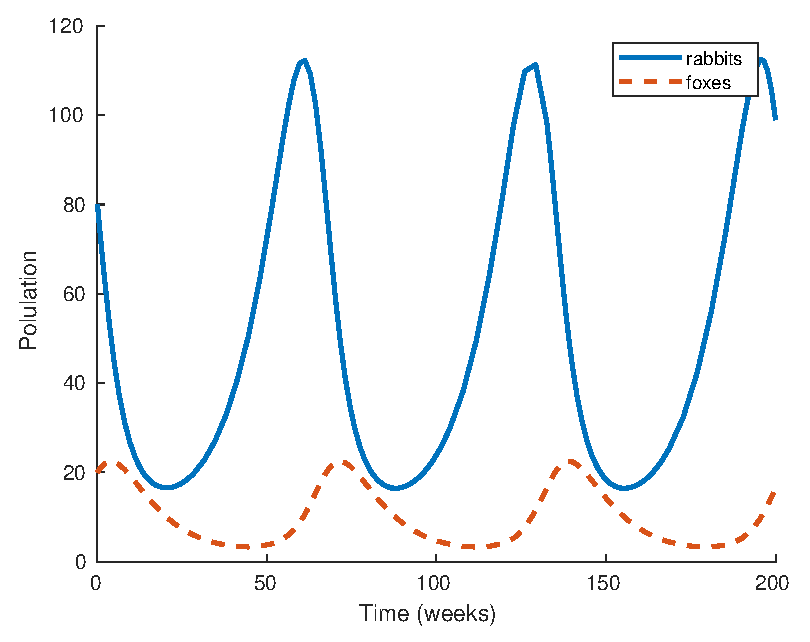
\includegraphics[height=3in]{book/figs/lotka.eps}}
\caption{Solution for the Lotka-Volterra model.}
\label{fig:lotka}
\end{figure}

Figure~\ref{fig:lotka} shows the results. The x-axis is time in weeks; the y-axis is population.  The top curve shows the population of rabbits; the bottom curve shows foxes.

\index{boom and bust}

Initially there are too many foxes, so the rabbit population declines.  Then there are not enough rabbits, and the fox population declines.  That allows the rabbit population to recover, and the pattern repeats.

This cycle of ``boom and bust'' is typical of the Lotka-Volterra model.


\subsection{Phase Plot}

Instead of plotting the two populations over time, it is sometimes useful to plot them against each other:

\begin{code}
>> ***plot(R, F)***
\end{code}
\begin{figure}[ht]

\centerline{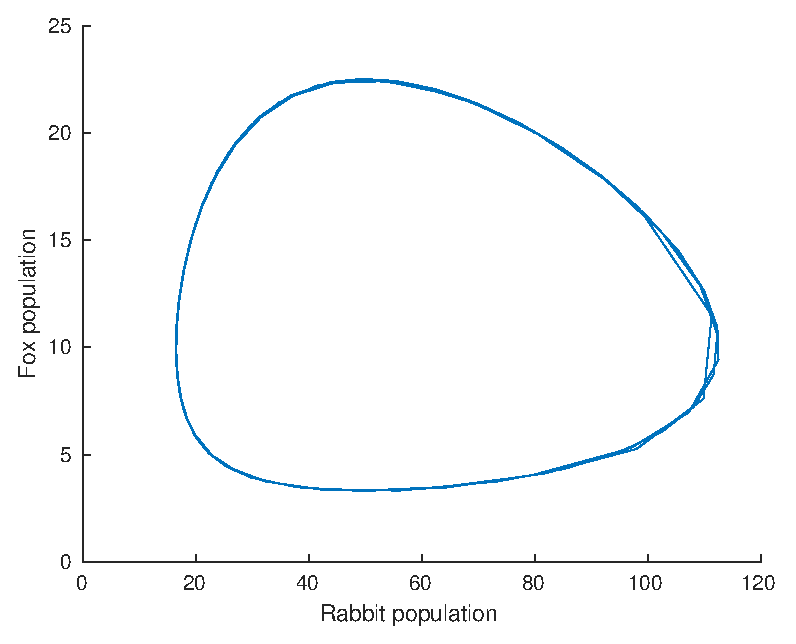
\includegraphics[height=3in]{book/figs/phase.eps}}
\caption{Phase plot from the Lotka-Volterra model.}
\label{fig:phase}
\end{figure}

Figure~\ref{fig:phase} shows the result.  
Each point on this plot represents a certain number of rabbits (on the
x axis) and a certain number of foxes (on the y axis).
Since these are the only two variables in the system, each point in
this plane describes the complete state of the system, that is, the values of
the variables we're solving for.

\index{phase plot}
\index{trajectory}
\index{state}

Over time, the state moves around the plane; Figure~\ref{fig:phase} shows
the path traced by the state over time; this path
is called a {\em trajectory}.

Since the behavior of this system is periodic, the trajectory is a loop.

If there are 3 variables in the system, we need 3 dimensions to show
the state of the system, so the trajectory is a 3-D curve.
You can use {\tt plot3} to trace trajectories in 3 dimensions,
but for 4 or more variables, you're on your own.

\index{plot3@{\tt plot3}}


\subsection{What Could Go Wrong?}

The output vector from the rate function has to be a column vector; otherwise you get an error:

\begin{code}
Error using odearguments (line 93)
RATE_FUNC must return a column vector.
\end{code}

Which is a pretty good error message.  It's not clear {\em why}
it needs to be a column vector, but that's not our problem.

\index{column vector}

Another possible error is reversing the order of the elements in the
initial conditions, or the vectors inside {\tt lotka}.  MATLAB
doesn't know what the elements are supposed to mean, so it can't catch
errors like this; it will just produce incorrect results.

The order of the elements (rabbits and foxes) is up to you, but
you have to be consistent.  That is, the order of the initial conditions you
provide when you call {\tt ode45} has to be the same as the order,
inside \verb"rate_func", where you unpack the input vector, and the
same as the order of the derivatives in the output vector.

\section{Chapter Review}

In this chapter, we used {\tt ode45} to solve a system of first order differential equations.
As an exercise, you'll have a chance to solve the famous Lorenz equations, one of the first examples of a chaotic system.

Here are the terms from this chapter you might want to remember.

A {\em row vector} is a matrix that has only one row, and a {\em column vector} is a matrix that has only one column.
The {\em transpose} operation transforms the rows of a matrix
into columns (or the other way around, if you prefer).

A {\em system of equations} is a collection of equations written in terms of
the same set of variables.

In a rate function, we often have to {\em unpack} the input variable,
copying the elements of a vector into a set of variables.
Then we have to {\em pack} the results into a vector as an output variable.

The {\em state} of a system is a set of variables that quantify the condition of the system as it changes over time.

When we solve a system of differential equations, we can visualize the results with a {\em phase plot}, which shows the state of a system as point in the space of possible states.
A {\em trajectory} is a path in a phase plot that shows how the state of a system changes over time.

In the next chapter, we move on to second-order systems, which we use to describe systems
with objects moving in space, governed by Newton's laws of motion.


\section{Exercises}

\begin{ex}

\index{Lorenz attractor}

Based on the examples we've seen so far, you'd think that all ODEs describe population as
a function of time, but that's not true.

According to Wikipedia, ``The Lorenz attractor, introduced by Edward Lorenz in 1963, is a
non-linear three-dimensional deterministic dynamical system derived
from the simplified equations of convection rolls arising in the
dynamical equations of the atmosphere. For a certain set of parameters
the system exhibits chaotic behavior and displays what is today called
a strange attractor...'' (see \url{https://greenteapress.com/matlab/lorenz}).

The system is described by this system of differential equations:
%
\begin{eqnarray}
x_t &=& \sigma (y - x)  \\
y_t &=& x (r - z) - y   \\
z_t &=& xy - b z
\end{eqnarray}
%
Common values for the parameters are $\sigma = 10$, $b = 8/3$, and $r=28$.

Use {\tt ode45} to estimate a solution to this system of equations.


\begin{enumerate}

\item Create a file named {\em lorentz.m} with a top-level function named {\tt lorenz} and a helper function named \verb"rate_func".

\item  The rate function should
takes {\tt t} and {\tt V} as input variables, where the components
of {\tt V} are understood to be the current values of {\tt x},
{\tt y} and {\tt z}.  It should compute the corresponding derivatives
and return them in a single column vector.

\item Test the function by calling it from the top-level function with values like $t=0$, $x=1$, $y=2$, and $z=3$.  
Once you get your function working, you should make it a silent function before calling {\tt ode45}.

\item Use {\tt ode45} to estimate the solution for the time span $[0, 30]$
with the initial condition $x=1$, $y=2$, and $z=3$.

\item Plot the results as a time series, that is, each of the variables as a function of time.

\item Use {\tt plot3} to plot the trajectory of $x$, $y$, and $z$.

\end{enumerate}

% lorenz.m
\end{ex}

